\documentclass[letterpaper, 10pt, conference]{IEEEconf}

\usepackage{amsmath,amsfonts}
\usepackage{array}
\usepackage{url}
\usepackage{graphicx}
\usepackage{cite}

\usepackage{color} % used for red comments
\usepackage[acronym]{glossaries} % acronyms

\usepackage[linesnumbered]{algorithm2e} % algorithms
\RestyleAlgo{ruled}

%===============================================================================
% acronynms ====================================================================
%===============================================================================

\newacronym{cnn}{CNN}{Convolutional Neural Networks}

\newacronym{dh}{DH}{Denavit-Hartenberg}
\newacronym[longplural={Dynamical Systems}]{ds}{DS}{Dynamical System}
\newacronym{dmp}{DMP}{Dynamic Movement Primitive}
\newacronym[longplural={Degrees of Freedom}]{dof}{DoF}{Degree of Freedom}
\newacronym{dl}{DL}{Deep Learning}


\newacronym{gan}{GAN}{Generative Adversarial Network}
\newacronym[longplural={Gausian Processes}]{gp}{GP}{Gaussian Process}
\newacronym[longplural={Graph Gausian Processes}]{ggp}{GGP}{Graph Gaussian Process}
\newacronym{gmm}{GMM}{Gaussian Mixture Model}
\newacronym{gpr}{GPR}{Gaussian Process Regression}

\newacronym{iil}{IIL}{Interactive Imitation Learning}

\newacronym{hmm}{HMM}{Hidden Markov Model}
\newacronym{hsmm}{HSMM}{Hidden Semi-Markov Model}

\newacronym{kt}{KT}{kinesthetic teaching}
\newacronym{kd}{KD}{kinesthetic demonstration}

\newacronym{lfd}{LfD}{Learning from Demonstrations}
\newacronym{lstm}{LSTM}{Long Short-Term Memory}
\newacronym{lwpr}{LWPR}{Locally Weighted Projection Regression}

\newacronym{pca}{PCA}{Principal Component Analysis}

\newacronym{mp}{MP}{Movement Primitive}

\newacronym{nn}{NN}{Neural Network}

\newacronym{rl}{RL}{Reinforcement Learning}
\newacronym{rbf}{RBF}{Radial Basis Function}

\newacronym{svr}{SVR}{Support Vector Regression}

\newacronym{tphsmm}{TPHSMM}{Task Parameterized Hidden Semi-Markov Model}
\newacronym{tpgmm}{TPGMM}{Task Parameterized Gaussian Mixture Model}

%%%%%%   TEMPLATE -------------------
\IEEEoverridecommandlockouts
\overrideIEEEmargins                                      % Needed to meet printer requirements.


%%%%%%%%%%%%%%%%%%%%%%%%%%%%%%%%%%%%
\graphicspath{{figures}}

\newcommand{\rev}[1]{\color{red}(#1)\color{black}}
\newcommand{\cn}{\rev{citation needed}}
%%%% Robot
\newcommand{\joint}[1]{\mathrm{J}_{#1}}
\newcommand{\rotAngle}[1]{q_{#1}}
\newcommand{\nJoints}{j}
\newcommand{\nDims}{n}
\newcommand{\pos}{x}
\newcommand{\jacob}{\matrix{J}}

% Network
\newcommand{\prediction}[1]{\tilde{#1}}
\newcommand{\nn}{\Phi}
\newcommand{\nnMono}{\nn^{m}}
\newcommand{\nnLink}{\nn^{l}}
\newcommand{\loss}{\mathcal{L}}
\newcommand{\lossMono}{\loss^{m}}
\newcommand{\lossLink}{\loss^{l}}
\newcommand{\lossLinkCart}{\loss^{l,cart}}
\newcommand{\lossLinkDet}{\loss^{l,det}}
\newcommand{\lossLinkInv}{\loss^{l,inv}}
\newcommand{\predMono}{\prediction{\vector{x}}^{m}}
\newcommand{\predLink}{\prediction{\vector{x}}^{l}}
\newcommand{\nLayers}{l_n}
\newcommand{\layerSize}{l_s}
\newcommand{\nParams}{|\nn|}
\newcommand{\learningRate}{lr}

% General math
\newcommand{\realSet}[1]{\mathbb{R}^{#1}}
\renewcommand{\matrix}[1]{\mathrm{\mathbf{#1}}}
\renewcommand{\vector}[1]{\mathrm{\mathbf{#1}}}
\newcommand{\normalDist}[2]{\mathcal{N}(#1, #2)}

% Learning
\newcommand{\epochs}{epochs}
\newcommand{\nSamples}{nSamples}
\newcommand{\memory}{mem}
\newcommand{\nIterations}{nIter}
\newcommand{\batchSize}{bs}
\newcommand{\meanLoss}{\bar{\loss}}

% Tuning
\newcommand{\lossTune}{\meanLoss^{tune}}

% RL
\newcommand{\policy}{\Pi}
\newcommand{\linksLenght}{\vector{d}}
\newcommand{\var}{\sigma}

%software
\newcommand{\softwareFont}[1]{\texttt{#1}\xspace}
\newcommand{\optuna}{\softwareFont{Optuna}}
\newcommand{\ray}{\softwareFont{Ray Tune}}
\newcommand{\zoo}{\softwareFont{RL-Zoo}}
\newcommand{\gym}{\softwareFont{Gym}}
\newcommand{\mujoco}{\softwareFont{MuJoCo}}
\newcommand{\torch}{\softwareFont{PyTorch}}
\newcommand{\autograd}{\softwareFont{Autograd}}
\newcommand{\sac}{\softwareFont{SAC}}
\renewcommand{\sb}{\softwareFont{Stable-baselines3}}

\hyphenation{op-tical net-works semi-conduc-tor IEEE-Xplore}
% updated with editorial comments 8/9/2021



\title{\LARGE \bf A DH-Transformation-Based Neural Network Architecture for Forward Kinematics Learning}

\author{Leandro de Souza Rosa$^{1}$, Luca Iocchi$^{1}$%
	\thanks{$^{1}$Department of Computer Engineering, Robotics and Management,
		Sapienza University of Rome, 00185 Rome, Italy
		{\tt\small leandro.desouzarosa@uniroma1.it, iocchi@diag.uniroma1.it}
	}%
}

\begin{document}

\maketitle
\thispagestyle{empty}
\pagestyle{empty}

\begin{abstract}
	...
\end{abstract}

\begin{IEEEkeywords}
	A, B, C.
\end{IEEEkeywords}


$  $\section{Introduction}\label{sec: introduction}

Forward kinematics is arguably one of the most basic computations in robotics, which provides means of computing the position of joints, or other links, in a chosen reference frame (often the world frame).
%
This computation is commonly found in Cartesian impedance \cite{schaffer2002cartesian} and compliance \cite{scherzinger2017forward} controllers, and also has seen recent application in collision detection \cite{das2020forward}.
%
For industrial and commercial robots, the forward kinematics is computed based on a detailed and accurate system description provided by the manufacturer.

Nevertheless, for low-cost or in-house-built robots, achieving a satisfactory forward kinematics is not a trivial task, and often learning-based methods are adopted. \cn

In order to learn forward kinematics, common approaches found in the literature often rely on using a monolithic \gls{nn} to approximate the mapping between joints and position, without giving much attention to the \gls{nn} architecture and its impacts in learning efficiency and final model precision.
%
Furthermore, little attention has been given for the learning scalability as the number of joints increase.

In this paper we propose a novel \gls{nn} architecture based on \gls{dh} transformations for learning forward kinematics.
%
The proposed architecture consists of one \gls{nn} for estimating the transformation of each joint with respect to the previous one, and leverages the chaining properties of \gls{dl} transformations for computing the forward kinematics with respect to a common reference frame.
 
In order to test the proposed architecture, we simulate robotic manipulators with $2$, up to $7$ joints, showing increasing gains in sampling efficiency and accuracy as the number of joints increase.
%
We further demonstrate the impacts of using the proposed architecture on higher level computations based on the forward kinematics, namely velocity estimation through Jacobian computation and on a \gls{rl} policy learning.
 
\section{Related Works}\label{sec: related works}

\cite{nguyen1990neural} probably the first proposal of learning forward kinematics with \gls{nn}. Uses a monolithic network and a planar 2-link robotic arm.

\cite{gribovskaya2011learning} proposes to learn forward kinematics as a monolithic \gls{gmm} model. They test on a real robot with \rev{3?}-\gls{dof}.

\cite{damas2012online} proposed to learn the forward and inverse kinematics together for parallel robots. The approach uses a monolithic model, which is learned online using a \gls{lwpr}.

\cite{morell2013solving} proposes to solve the forward kinematics using \gls{svr}.

\cite{gu2017deep} proposes to learn a policy with deep-Q learning. They use simulation and robot farms. (fells like I`ve the images of this paper in another paper. double check)

\cite{kubus2018learning} presents as analysis on sample efficiency for learning the forward kinematics of linked robots. Using tailored parameterized models is efficient, other methods are not sample efficient. They focus on Fourier-Domain representations.

\cite{theofanidis2018kinematic} solves the forward kinematics of a 6-\gls{dof} serial manipulator using a monolithic \gls{nn}.

\cite{grassmann2019merits} study the influence of joint-position representations on learning forward kinematics with a monolithic \gls{nn} for a 6-\gls{dof} robotic arm and a cylindrical robot. They test \texttt{Euler angles}, \texttt{vectorial}, \texttt{quaternions}, and \texttt{angle-axis} representation. Results favor quaternion representation.

\cite{ren2020learning} proposes learning the inverse kinematics and the dynamics model of serial robot manipulators using \glspl{gan}.

\cite{loutfi2020learning} evaluates different function approximators for learning monolithic forward kinematic models. \glspl{nn} perform the best.

\cite{dalla2020autonomous} uses \gls{gpr} for learning the forward kinematics based on vision. The approach considers a monolithic \gls{gp}.

\cite{kesaba2022transfer} uses a monolithic \gls{nn} for learning forward kinematics for a 6-\gls{dof} robot manipulator in simulation. The learned model is transferred to a real robot \rev{using the same training signals}. Results show that the real robot achieves higher accuracy.

\cite{kesaba2022forward} seems to be the same as \cite{kesaba2022transfer}.

\cite{sharkawy2022forward} uses a monolithic \gls{nn} for learning forward and inverse kinematics of a 5-\gls{dof} robotic arm \rev{check it out it seems they do it for 2 DoFs}. 

\cite{valayil2022methods} basically lists methods for solving forward kinematics. \rev{does not really add anything}

\cite{sharkawy2023forward} uses a monolithic \gls{nn} for learning forward kinematics of a 3-\gls{dof} robotic arm. 
\section{Preliminaries}\label{sec: preliminaries}

Consider the serial robot manipulator illustrated in Figure \ref{fig: serial manipulator} with $\nJoints$ links and $\nJoints+1$ joints. 
%
The reference frames of the world and of $\joint{0}$ are fixed and coincide.

\begin{figure}
	\centering
	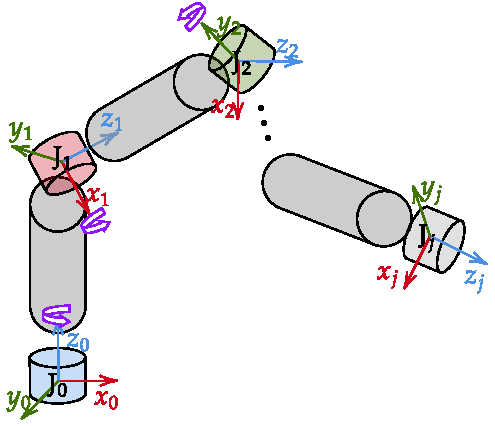
\includegraphics[width=0.8\linewidth]{serial_manipulator.pdf}
	\caption{A serial manipulator with $\nJoints$ axes and $\nJoints+1$ joints $\joint{i}$. Each axis is connected by a joint which is associated with a Cartesian reference frame (red, gree, blue) and can rotate over an arbitrary axis (purple).
	%
	We consider, without loss of generality, the position of $\joint{0}$ fixed at the world origin, and $\joint{\nJoints}$ to be the end-effector, which does not rotate.
	%
	The Cartesian position of joint $\joint{i}|i \in\{1,\hdots,\nJoints\}$ ($\vector{x}_i$) in the reference frame of $\joint{i_1}$ depends only on $\rotAngle{i-1}$.
	}
	\label{fig: serial manipulator}
\end{figure}

Our task is to estimate the Cartesian position of each joint $\joint{i}|i\in\{1,\hdots,\nJoints\}$ in the world reference frame ($\vector{x}$) as a function of the rotation angles of $\joint{i}|i\in\{0,\hdots,\nJoints-1\}$ ($\rotAngle{i}|i\in\{0,\hdots,\nJoints-1\}$), as described in Equation \ref{eq: x estimate in function of q}.
%
The Cartesian pose of each joint $\joint{i}$ is a $d$ dimensional array (usually $\nDims=2, 3$), resulting in the estimation of $\nDims\times\nJoints$ functions in total.

\begin{equation}\label{eq: x estimate in function of q}
	\prediction{\vector{x}}(\vector{q}) = 
	\left[
	\begin{array}{cccc}
		\prediction{\vector{x}}_1(\rotAngle{0}) & \prediction{\vector{x}}_2(\rotAngle{0}, \rotAngle{1}) & \hdots & \prediction{\vector{x}}_\nJoints(\rotAngle{0}, \hdots, \rotAngle{\nJoints-1})
	\end{array}
	\right]
\end{equation}

The function $\vector{x}(\vector{q})$ can be expressed using \gls{dh} transformation matrices \cite{kucuk2006robot}.
%
For a given $\joint{i}$, the a transformation between its reference frame and the one of $\joint{i-1}$ is described by \ref{eq: dl transformation matrix i-1 to i}, where $\matrix{T}$ and $\matrix{D}$ are the rotation and displacement matrices, respectively.

\begin{equation}\label{eq: dl transformation matrix i-1 to i}
	\matrix{T}_{i-1}^{i} = 
	\left[
	\begin{array}{cc}
		\matrix{R}_{i-1}^{i}(\rotAngle{i-1}) & \matrix{D}_{i-1}^{i}(\rotAngle{i-1}) \\
		\matrix{0}_{1\times3} & 1
	\end{array}
	\right]
\end{equation}

For a serial manipulator, the transformations can be chained for obtaining a transformation for any given joint $\joint{i}$ in the world reference frame, according to Equation \ref{eq: dl transformation matrix 0 to i}.

\begin{equation}\label{eq: dl transformation matrix 0 to i}
	\matrix{T}^i_0 = \displaystyle\prod_{k=1}^{i}\matrix{T}_{k-1}^{k}~|~i \in \{1, \hdots, j\}
\end{equation}
\section{Proposed Architecture}\label{seec: proposed architecture}

\subsection{Overview}\label{subsec: overview}

While approaches in the literature propose to learn a monolithic approximator $\predMono = \nnMono(\vector{\rotAngle{}}):\realSet{\nJoints}\rightarrow\realSet{\nDims\times\nJoints}$, our main idea is to learn one approximator for each joint $\joint{i}$, which encodes $\matrix{T}_{i-1}^{i}$, and thus learning $\nJoints$ predictors $\predLink_i = \nnLink_i(\vector{\rotAngle{i}}):\realSet{1}\rightarrow\realSet{\nDims\times(\nDims+1)}~|~i\in\{1,\hdots\nJoints\}$, and joining all $\nnLink_i$ leads to the proposed model $\nnLink$.


\begin{figure}
	\centering
	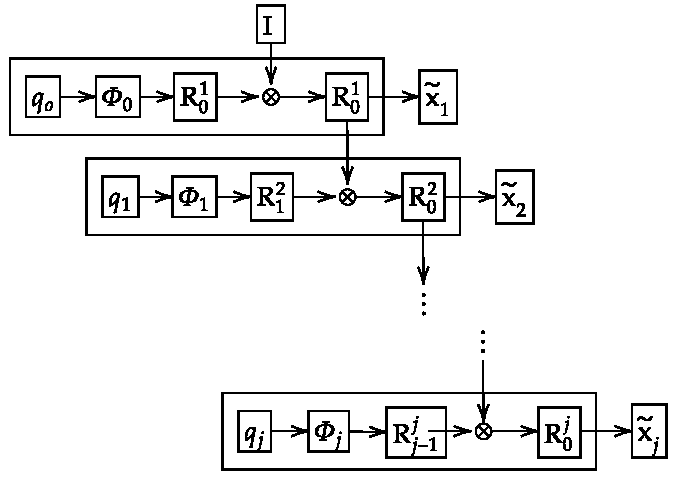
\includegraphics[width=\linewidth]{linked_network_overview.pdf}
	\caption{Proposed architecture. For each joint $i\in\{1,\hdots,j\}$, a network $\nnLink_i$ learns the \gls{dh} transformation from joint $i-1$ to $i$ $\matrix{R}_{i-1}^{i}$.
	%
	$\matrix{R}_{i-1}^{i}$ is multiplied by the cumulative transformation of all previous joints, resulting in $\matrix{R}_{0}^{i}$, from which the Cartesian position of joint $i$ $\prediction{\vector{x}}_i$ is obtained directly.}
	\label{fig:linked network overview}
\end{figure}

\subsection{Loss Function}\label{subsec: loss}

For training $\nn$, we follow the approaches in the literature \rev{citation needed} and use the average Euclidean distance between the joints and their respective prediction, as described in Equation \ref{eq: loss}.
%
Note that some approaches in the literature consider only the end-effector position and its prediction, which is reasonable since in a real robot, the position of individual joints is hard to obtain, while the end-effector's position can be obtained with off-the-shelf trackers and cameras \rev{citation}.
%
In contrast, since we perform the training in simulation, we have the flexibility of considering all joints, leading to a richer loss signal, improving the training convergence.

\begin{equation}\label{eq: loss}
	\loss = \frac{1}{\nJoints}\sum_{k=1}^{\nJoints}||\prediction{x}_k-\vector{x}_k||
\end{equation}

%Similarly, for each $\nnLink_i$, we average the Euclidean distance between for all joints up to $\joint{i}$, according to Equation \ref{eq: loss link cart}.
%\begin{equation}\label{eq: loss link cart}
%	\lossLinkCart_i = \frac{1}{i}\sum_{k=1}^{i}||\predMono_k-\vector{x}_k|| ~|~ i\in\{1,\hdots,j\}
%\end{equation}
%Furthermore, we explore two properties of rotation matrices by adding two extra loss terms for $\nnLink_i$.
%
%The first property is that $\det(\matrix{R}) = 1$, which is captured by Equation \ref{eq: loss link det}.
%
%The second property is that $\matrix{R}^{T} = \matrix{R}^{-1}$, which is capture by Equation \ref{eq: loss link inv}.
%\begin{equation}\label{eq: loss link det}
%	\lossLinkDet_i = ||\det(\prediction{\matrix{R}}_i) - 1|| ~|~ i\in\{1,\hdots,j\}
%\end{equation}
%
%\begin{equation}\label{eq: loss link inv}
%	\lossLinkInv_i = ||\prediction{\matrix{R}}_i\prediction{\matrix{R}}_i^{T} - \matrix{I}|| ~|~ i\in\{1,\hdots,j\}
%\end{equation}
%The final loss for training $\nnLink_i$ is given by Equation \ref{eq: loss link}.
%
%The reason for incorporating $\lossLinkInv_i$ and $\lossLinkDet_i$ in $\lossLink_i$ is to motivate $\nnLink_i$ to converge to valid \gls{dh} matrices, indirectly pushing $\prediction{\matrix{D}}_i$ to converge to the proper Cartesian position of $\joint{i}$. 
%\begin{equation}\label{eq: loss link}
%	\lossLink_i = \lossLinkCart_i+\lossLinkInv_i+\lossLinkDet_i
%\end{equation}

\subsection{Training Procedure}\label{subsec: training procedure}

Since in this stage we use simulation, both $\nnMono$ and $\nnLink$ are trained in a straight-forward 
fashion according to Algorithm \ref{alg: train nn}.
%
For each epoch of training, $nSamples$ random poses are sampled in joint space (line $3$), and the respective Cartesian position of each joint is obtained directly from the simulator (line $4$) and added to a memory buffer (line $5$).
%
The memory size is limited, and upon additions further than its limit, it drops a percentage of its oldest data (we use a $10\%$ data drop in all experiments) for reducing data allocation overheads.
%
Next, $nIterations$ of training is done with the data already within the memory, which are done by randomly sampling $batchSize$ samples from the memory (line $8$), computing the average loss (lines $9$ to $13$), which is then back-propagated through the network (line $14$).
 
\begin{algorithm}
	\caption{Training procedure for $\nn$.}\label{alg: train nn}
	\For{$e \in \{1,\hdots, epochs\}$}{
		\For{$r \in \{1,\hdots, nSamples\}$}{
			$q\leftarrow$ random joint positions\;
			$x\leftarrow$ Cartesian position of all joints given $q$\;
			add $(q, x)$ to $memory$\;
		}
		
		\For{$t\in\{1,\hdots,nIterations\}$}{
			$(qs, xs)\leftarrow$ get $batchSize$ random samples from $memory$\; 
			$meanLoss\leftarrow0$\;
			\For{$(q, x) \in (qs, xs)$}{
				$meanLoss\leftarrow acc+\loss$\;
			}
			$meanLoss\leftarrow acc/batchSize$\;
			backpropagate $meanLoss$ through $\nn$\; 
		}
	}
\end{algorithm}

It is worthy to notice that in our tests, we observed that randomly sampling poses leads to a much higher efficiency than performing random walks, which is to be expected due to the better state space coverage. 
%
However, when considering a real robot in the \gls{rl} loop, it is unpractical to sample the state space this way, since the robot will be naturally performing a random walk.
%
In section \ref{sec: rl case of study}, we present a \gls{rl} case of study highlighting the proposed architecture impacts in this scope.
\section{Results}\label{sec: results}

\subsection{Testing Environment}\label{subsec: test env}

We build upon the \texttt{Reacher} environment from OpenAI Gym \cite{gym}, which consists of a 2D serial manipulator with $2$ joints simulated using MuJoCo \cite{todorov2012mujoco}.
%
In order to evaluate the proposed approach for more realistic robots, we extend the environment enabling for 3D, and adding models for robots up to $7$ joints\footnote{Publicly available source code: \href{https://github.com/lsrosa/kinematics\_learning}{https://github.com/lsrosa/kinematics\_learning}}.

We implement $\nnMono$ and $\nnLink$ as feed-forward \gls{nn}.
%
While other approximators could be used, e.g., \glspl{gp} as in \cite{dalla2020autonomous}, their evaluation falls out-of-the-scope of this paper.

\subsection{Tuning $\nn$}\label{subsec: tuning}

In order to assure appropriate hyper-parameters for $\nn$, we perform a tuning for each model, which results in the values presented in Table \ref{tab: tune fkine}, where $lr$ is the learning rate, and \texttt{arch} is an array containing the number of elements neurons in each \gls{nn} layer. 
%
For the learning hyper-parameter of Algorithm \ref{alg: train nn}, we found that $nSamples=1e^3$, $epochs=500$, $nIterations=50$, $batchSize=100$ are adequate values for all networks.

\begin{table}
	\centering
	\begin{tabulary}{\linewidth}{c|c|c|c|c|c|c|c}
		\toprule
		\multicolumn{8}{c}{$\nDims=2$} \\\hline
		$\nJoints$ & 1 & 2 & 3 & 4 & 5 & 6 & 7 \\\midrule
		$lr$ & & & & & & & \\\hline
		$\nnMono$ \texttt{arch} & & & & & & & \\
		\midrule
		\multicolumn{8}{c}{$\nDims=3$} \\\hline
		$lr$ & & & & & & & \\\hline
		$\nnMono$ \texttt{arch} & & & & & & & \\
		\midrule
		\midrule
		\multicolumn{8}{c}{$\nDims=2$} \\\hline
		$lr$ & & & & & & & \\\hline
		$\nnLink$ \texttt{arch} & & & & & & & \\
		\midrule
		\multicolumn{8}{c}{$\nDims=3$} \\\hline
		$lr$ & & & & & & & \\\hline
		$\nnLink$ \texttt{arch} & & & & & & & \\
		\bottomrule
	\end{tabulary}
	\caption{Tuning parameters for 2D and 3D robots with varying number of joints.}
	\label{tab: tune fkine}
\end{table}

\subsection{Loss and Accuracy Results}

Figure \ref{fig: loss fkines} presents the losses when learning $\nnMono$ and $\nnLink$, which shows that the proposed architecture outperforms the monolithic approach found used in the literature.

\begin{figure*}
	\includegraphics[width=\textwidth, height=2in]{example-image-a}
	\caption{Loss comparison between $\nnMono$ and $\nnLink$. The solid line and shaded area represent the mean loss and the area between minimum and maximum losses over $30$ trials.}
	\label{fig: loss fkines}
\end{figure*}

For qualitative comparison, Figure \ref{fig: joints position} presents the joints position estimation obtained by $\nnMono$ and $\nnLink$, in which the higher accuracy can be seem.

\begin{figure*}
	\includegraphics[width=\textwidth, height=2in]{example-image-a}
	\caption{Joints position estimation comparison for $\nnMono$ and $\nnLink$.}
	\label{fig: joints position}
\end{figure*}

Next, to demonstrate the accuracy impacts, we estimate the end-effector velocity $\dot{\pos}_j = \left[\jacob\dot{\rotAngle{}}\right]_j$, where $\jacob$ is the unknown Jacobian matrix of the robot, as $\prediction{\dot{\pos}}_j = \left[\frac{\partial\nn}{\partial\rotAngle{}}\right]_j$.
%
Figure \ref{fig: ee vel} shows the velocity estimation and ground-truth obtained from the simulator for $\nDims=3$ and $\nJoints=7$ only, while for the 2D and other joint number cases are omitted for briefness.

\begin{figure}
	\includegraphics[width=\linewidth]{example-image-a}
	\caption{End-effector velocity estimation comparison for $\nnMono$ and $\nnLink$.}
	\label{fig: ee vel}
\end{figure}
%\section{Reinforcement Learning Case of Study}\label{sec: rl case of study}

This section presents a case of study using the forward kinematics estimation in a \gls{rl} loop, which consists of two steps.
%
In the fist step, we train $\nn$ and a policy $\policy:\realSet{\nDims\times\nJoints}\rightarrow\realSet{\nJoints}$, which given the Cartesian position of the robot joints, learns the torques for each joint for moving the end-effector towards the target position, using the pre-trained $\nn$ model learned in Section \ref{sec: results} for estimating $\vector{\pos} = \nn(\vector{\rotAngle{}})$.
%
In the second step, we create a different robot with the same number of joints, by varying its links' dimension according to a normal distribution $\normalDist{\linksLenght}{\var=0.01}$, where $\linksLenght$ is the dimensions of the robot used in the first step, and retrain both $\nn$ and $\policy$ on the new robot.
%
As such, $\policy$ encompasses learning the robot's dynamics, and control, which is a considerably hard task for high-dimensions.

This study case mimics a straight-forward transfer-learning case, in which first a model is firstly trained in simulation, and then refined in a real robot, which is slightly different from the simulated one.
%
These differences may come from imprecise measures, or from an unknown model, as in the case of budget robot manipulators \cite{zajc2022low}. 
%
Furthermore, more elaborated transfer-learning approaches \cite{stuber2018feature,bocsi2013alignment} might also benefit from the proposed network, but its evaluation falls out-or-the-scope with this paper.

The results in this section are limited to the 3D and a robot with $7$ joints, and the second part of the learning is also done in simulation. 
%
%This limitation is due to the extensive long time necessary to tune, and learn $\policy$, and then to adapt both $\nn$ and $\policy$ to the new environment, since in the \gls{rl} loop, the reward is sparse and the robot performs a random-walk sampling.

For $\policy$ we use a \sac from \sb \cite{stablebaselines3}, and $\nn$ is introduced into the \sac as such its outputs are the inputs of \sac's features extraction step. 
Figure \ref{fig: learn and adapt policy} presents the rewards obtained in both steps, where we can see...

\begin{figure}
	\includegraphics[width=\linewidth]{example-image-a}
	\caption{Reward for learning $\policy$ using the pre-trained $\nn$, and for adapting $\policy$ to the modified robot using.}
	\label{fig: learn and adapt policy}
\end{figure}

\section{Conclusions}\label{sec: conclusions}

This paper presents a novel \gls{nn} architecture for learning the forward kinematics of serial robot manipulators.
%
Instead of a monolithic approach in which the joints positions are estimated with a relatively large \gls{nn}, the proposed architecture leverages the \gls{dh}-Transformation notation, resulting in a link-by-link estimator and keeping a constant complexity for the estimation between links.

Results show that the proposed architecture improves the learning efficiency, regarding to the number of samples, and achieves better precision when compared to the traditional monolithic approach found in the literature.
%
Furthermore, the proposed architecture is shown scale better for robots with increasing number of joints.
 

\section*{Acknowledgements}
This work has been supported by the PNRR MUR project PE0000013-FAIR

\bibliographystyle{IEEEtran}
\bibliography{biblio/biblio}

%\begin{IEEEbiography}[{\includegraphics[width=1in,height=1.25in,clip,keepaspectratio]{fig1}}]{Michael Shell}
	Use $\backslash${\tt{begin\{IEEEbiography\}}} and then for the 1st argument use $\backslash${\tt{includegraphics}} to declare and link the author photo.
	Use the author name as the 3rd argument followed by the biography text.
\end{IEEEbiography}

\vspace{11pt}

\bf{If you will not include a photo:}\vspace{-33pt}
\begin{IEEEbiographynophoto}{John Doe}
	Use $\backslash${\tt{begin\{IEEEbiographynophoto\}}} and the author name as the argument followed by the biography text.
\end{IEEEbiographynophoto}

\vfill

\end{document}


